\documentclass[12pt]{article}

% --- Packages ---
\usepackage[a4paper, margin=1in]{geometry}
\usepackage{graphicx}
\usepackage{setspace}
\usepackage{times}
\usepackage{array}
\usepackage{caption}
\usepackage{microtype}
\usepackage{float}
\usepackage{titlesec}
\usepackage{enumitem}
\usepackage{booktabs}
\usepackage{amsmath}
\usepackage{amssymb}
\usepackage{multirow}
\usepackage{xcolor}
\usepackage{xurl}
\usepackage{hyperref} % hyperref should be loaded last (or near last)

% --- Hyperref Setup ---
\hypersetup{
    colorlinks=true,
    linkcolor=blue!70!black,
    urlcolor=blue!70!black,
    citecolor=blue!70!black,
    pdftitle={Breast Cancer Detection using Ensemble Learning - Phase I Report},
    pdfauthor={VIT Bhopal University},
}

% --- Setup ---
\setstretch{1.1}
\pagestyle{plain}
\sloppy

% Format Section Headings
\titleformat{\section}{\fontsize{14}{16}\bfseries\uppercase}{\thesection.}{1em}{}
\titleformat{\subsection}{\fontsize{12}{14}\bfseries}{\thesubsection}{1em}{}

\begin{document}

%==================== 1. TITLE PAGE ====================%
\begin{titlepage}
    \centering
    \vspace*{0.5cm}
    
    {\fontsize{18}{22}\selectfont \textbf{Breast Cancer Detection using Ensemble Learning} \par}
    
    \vspace{1.5cm}
    
    {\fontsize{14}{18}\selectfont \textbf{An Engineering Project in Community Service} \par}
    
    \vspace{0.3cm}
    
    {\large \textbf{Phase -- I Report} \par}
    
    \vspace{0.8cm}
    
    {\large \textit{Submitted by} \par}
    
    \vspace{0.8cm}
    
    \begin{tabular}{clc}
        \toprule
        \textbf{Sl. No.} & \textbf{Register Number} & \textbf{Name} \\ 
        \midrule
        1 & 23BEC10069 & Bhavya Sharma \\
        2 & 23BCE11634 & Suryanshi Ranawat \\
        3 & 23BEC10079 & Ujjwal Mishra \\
        4 & 23BCE11385 & Medhansh Singh Kushwaha \\
        5 & 23BAI11250 & Soumyadeep Chakravarti \\
        \bottomrule
    \end{tabular}
    
    \vspace{1.5cm}
    
    \begin{figure}[H]
        \centering
        
\includegraphics[width=0.6\textwidth]{Assets/VIT_LOGO.png}
    \end{figure}
    
    {\large \textit{in partial fulfillment of the requirements for the degree of} \par}
    
    \vspace{0.5cm}
    
    {\large \textbf{Bachelor of Technology} \par}
    
    \vfill
    
    \textbf{VIT Bhopal University} \\
    \textbf{Bhopal} \\
    \textbf{Madhya Pradesh} \\
    
    \vspace{1cm}
    
    {\large \textbf{February, 2026}}
    
\end{titlepage}

%==================== FRONT MATTER ====================%
\newpage
\pagenumbering{roman}

%==================== 2. BONAFIDE CERTIFICATE ====================%
\begin{figure}[H]
    \centering
    
\includegraphics[width=0.4\textwidth]{Assets/VIT_LOGO.png}
\end{figure}
\begin{center}
    \textbf{\Large Bonafide Certificate}
\end{center}
\vspace{1cm}

\noindent Certified that this project report titled \textbf{``Breast Cancer Detection using Ensemble Learning''} is the bonafide work of \textbf{``23BEC10069 Bhavya Sharma, 23BCE11634 Suryanshi Ranawat, 23BEC10079 Ujjwal Mishra, 23BCE11385 Medhansh Singh Kushwaha, 23BAI11250 Soumyadeep Chakravarti''} who carried out the project work under my supervision.

\vspace{1cm}

\noindent This project report (Phase I) is submitted for the Project Viva-Voce examination held on \dotfill

\vspace{2cm}

\begin{flushright}
    \textbf{Supervisor} \\
    Dr. Praveen Lalwani
\end{flushright}

\vspace{2cm}

\noindent
\begin{tabular}{p{0.45\textwidth}p{0.45\textwidth}}
    \textbf{Mrs. PAVITHRA R} & \textbf{Dr. Ujjwal Kumar Mishra} \\
    Comments \& Signature & Comments \& Signature \\
\end{tabular}

%==================== 3. DECLARATION ====================%
\newpage
\begin{center}
    \textbf{\Large Declaration of Originality}
\end{center}

\vspace{1cm}

\noindent We, hereby declare that this report entitled \textbf{``Breast Cancer Detection using Ensemble Learning''} represents our original work carried out for the EPICS project as a student of VIT Bhopal University and, to the best of our knowledge, it contains no material previously published or written by another person, nor any material presented for the award of any other degree or diploma of VIT Bhopal University or any other institution. Works of other authors cited in this report have been duly acknowledged under the section ``References''.

\vspace{2cm}

\noindent \textbf{Date:} 12 February 2026 \hfill \textbf{Reg No \& Name} \\
\null \hfill 23BEC10069 - Bhavya Sharma \\
\null \hfill 23BCE11634 - Suryanshi Ranawat \\
\null \hfill 23BEC10079 - Ujjwal Mishra \\
\null \hfill 23BCE11385 - Medhansh Singh Kushwaha \\
\null \hfill 23BAI11250 - Soumyadeep Chakravarti \\
\null \hfill (also signed by all students)

%==================== 4. ACKNOWLEDGEMENT ====================%
\newpage
\begin{center}
    \textbf{\Large Acknowledgement}
\end{center}

\vspace{1cm}

\noindent This work, has benefited in various ways from several people. Whilst it would be simple to name them all, it would not be easy to thank them enough.

\vspace{0.5cm}

\noindent I am deeply indebted to Dr. G. Viswanathan, Chancellor of VIT Bhopal University, and Dr. T. B. Sridharan, Pro Vice-Chancellor, VIT Bhopal University, for their unwavering support and guidance. Their leadership and vision have been a constant source of inspiration throughout my academic journey.

\vspace{0.5cm}

\noindent I would like to express my sincere gratitude to my supervisor, Dr. Praveen Lalwani, whose constant support, patience, and expertise were instrumental in completing this project. His guidance, valuable suggestions, and continuous encouragement helped me overcome challenges and successfully accomplish this research work.

\vspace{0.5cm}

\noindent I also extend my sincere thanks to Mrs. Pavithra R and Dr. Ujjwal Kumar Mishra for serving as reviewers and for their valuable feedback, constructive suggestions, and insightful comments, which greatly helped in improving the quality of this project.

\vspace{0.5cm}

\noindent I would also like to acknowledge the faculty members and staff of VIT Bhopal University who provided the necessary academic environment, resources, and support that facilitated the successful completion of this research work.

\vspace{0.5cm}

\noindent Lastly, I extend my deepest gratitude to my parents and friends, whose unwavering encouragement and support have been my driving force throughout this research endeavor. Their belief in me has been a source of strength and motivation.

%==================== 5. ABSTRACT ====================%
\newpage
\begin{center}
    \textbf{\Large Abstract}
\end{center}

\vspace{1cm}

\noindent Breast cancer is one of the most common and life-threatening diseases affecting women worldwide. Early and accurate detection plays a crucial role in improving patient survival rates and enabling effective treatment. Traditional diagnostic methods rely heavily on manual analysis by medical experts, which can be time-consuming and prone to human error. With the advancement of machine learning techniques, automated systems have been developed to assist in the early detection and classification of breast cancer.

\vspace{0.3cm}

\noindent This project presents a machine learning-based approach for breast cancer detection using ensemble learning techniques. Ensemble learning combines the predictions of multiple machine learning models to improve classification performance, accuracy, and reliability compared to individual models. In this work, several algorithms such as Decision Trees, Random Forest, and other classification techniques are utilized and combined to build a robust predictive model.

\vspace{0.3cm}

\noindent The system is trained and tested using a well-known medical dataset, the Wisconsin Breast Cancer Dataset, which contains various diagnostic features extracted from digitized images of breast masses. The dataset includes multiple attributes such as radius, texture, perimeter, area, and smoothness that help in distinguishing between benign and malignant tumors. Data preprocessing, feature analysis, and model training are performed to enhance prediction performance.

\vspace{0.3cm}

\noindent Experimental results demonstrate that ensemble learning techniques significantly improve classification accuracy and reduce misclassification rates compared to traditional single-model approaches. The proposed system provides a reliable and efficient method for assisting medical professionals in the early detection of breast cancer.

\vspace{0.3cm}

\noindent The implementation of such intelligent diagnostic systems can support healthcare providers in making faster and more accurate decisions, ultimately contributing to improved patient outcomes and more effective healthcare services.

\vspace{0.5cm}

\noindent \textbf{Keywords:} Breast Cancer Detection, Machine Learning, Ensemble Learning, Classification, Healthcare Analytics

%==================== 6. TABLE OF CONTENTS ====================%
\newpage
\tableofcontents

\newpage
\listoftables

%==================== MAIN CONTENT ====================%
\newpage
\pagenumbering{arabic}

\section{Introduction}

Breast cancer is one of the most common and serious diseases affecting women worldwide. It occurs when abnormal cells in the breast grow uncontrollably and form a tumor. Early detection of breast cancer is extremely important because it significantly increases the chances of successful treatment and survival. Traditional diagnostic methods such as mammography, biopsy, and clinical examination require expert interpretation and can sometimes lead to delays or inaccuracies in diagnosis.

With the rapid advancement of artificial intelligence and machine learning techniques, automated systems are being developed to assist medical professionals in diagnosing diseases more efficiently. Machine learning algorithms can analyze large amounts of medical data and identify hidden patterns that may not be easily detected by humans. These techniques can improve the speed, accuracy, and reliability of cancer detection.

This project focuses on developing a breast cancer detection system using ensemble learning methods. Ensemble learning combines multiple machine learning models to improve prediction performance and reduce errors compared to individual models. By integrating different classifiers, the system can provide more accurate and reliable predictions for identifying whether a tumor is benign or malignant.

The model is trained and evaluated using the Wisconsin Breast Cancer Dataset, which contains various features extracted from digitized images of breast tumors. These features include radius, texture, perimeter, area, and smoothness. By applying ensemble learning techniques to this dataset, the proposed system aims to improve diagnostic accuracy and assist healthcare professionals in making informed decisions.

\subsection{Motivation}

Breast cancer has become a major health concern across the world, affecting millions of women every year. Early detection plays a critical role in improving treatment outcomes and reducing mortality rates. However, traditional diagnostic methods can sometimes be time-consuming, expensive, and dependent on the experience of medical experts.

The motivation behind this project is to develop an intelligent system that can assist in the early detection of breast cancer using machine learning techniques. With the increasing availability of medical datasets and computational resources, machine learning models can analyze complex patterns in medical data and provide accurate predictions.

Ensemble learning methods are particularly powerful because they combine the strengths of multiple algorithms to produce better results than individual models. By implementing ensemble techniques, this project aims to create a more reliable and efficient system for breast cancer detection, which can support healthcare professionals and contribute to improved patient care.

\subsection{Objective}

The primary objective of this project is to develop an accurate and efficient system for the early detection of breast cancer using machine learning techniques. The project aims to analyze medical data and identify patterns that can help classify tumors as benign or malignant. By utilizing the Wisconsin Breast Cancer Dataset, the study focuses on understanding important tumor features such as radius, texture, perimeter, and smoothness that contribute to cancer diagnosis.

Another key objective is to implement and evaluate different machine learning algorithms and apply ensemble learning methods to improve the overall prediction performance. Ensemble techniques combine multiple models to enhance accuracy, reduce classification errors, and increase the reliability of the system.

Through comparative analysis of individual models and ensemble models, the project aims to determine the most effective approach for breast cancer prediction. Ultimately, the goal is to develop a reliable decision-support system that can assist healthcare professionals in diagnosing breast cancer at an early stage and contribute to improved patient outcomes.

%==================== SECTION 2: EXISTING WORK ====================%
\newpage
\section{Existing Work / Literature Review}

\subsection{Breast Cancer Diagnosis Using Machine Learning}

This study explores the use of several machine learning algorithms for breast cancer diagnosis using the Wisconsin Breast Cancer Dataset. The authors compared algorithms such as Support Vector Machine, Decision Tree, and Logistic Regression. Among these models, Support Vector Machine achieved the highest classification accuracy of approximately 96\%, demonstrating the effectiveness of machine learning techniques in medical diagnosis.

\subsection{Breast Cancer Prediction Using Random Forest}

This research focuses on the application of the ensemble learning algorithm Random Forest for breast cancer classification. Random Forest combines multiple decision trees to improve prediction accuracy and reduce overfitting. The model achieved an accuracy of around 97\% on the Wisconsin Breast Cancer Dataset, showing that ensemble methods can significantly improve diagnostic performance.

\subsection{Breast Cancer Detection Using Support Vector Machine}

In this work, the authors applied Support Vector Machine to classify tumors as benign or malignant. The model uses a hyperplane to separate classes based on extracted tumor features such as radius, texture, and smoothness. Experimental results showed high accuracy and reliability in detecting breast cancer cases.

\subsection{Breast Cancer Classification Using Neural Networks}

This study investigates the use of Artificial Neural Network models for breast cancer detection. Neural networks learn complex relationships between features and classification labels. The proposed model achieved an accuracy of approximately 95--97\%, demonstrating the capability of deep learning methods in medical diagnosis.

\subsection{Breast Cancer Prediction Using Ensemble Learning}

This research combines multiple classifiers using ensemble techniques such as voting and bagging. Algorithms including Decision Trees, Random Forest, and Logistic Regression were integrated to improve prediction performance. The ensemble approach achieved higher accuracy compared to individual models.

\subsection{Breast Cancer Detection Using Gradient Boosting}

This study applies the boosting-based algorithm Gradient Boosting to improve classification performance. Boosting sequentially trains models by focusing on previously misclassified samples. The results showed improved accuracy and reduced error rates in breast cancer prediction.

\subsection{Breast Cancer Diagnosis Using XGBoost}

The authors used the powerful ensemble algorithm XGBoost for breast cancer classification. XGBoost improves performance by optimizing gradient boosting techniques. The model achieved accuracy greater than 97\% and showed strong predictive performance compared to traditional classifiers.

\subsection{Breast Cancer Detection Using Deep Learning}

This research explores the use of deep learning methods for analyzing medical data and identifying cancerous tumors. Convolutional neural networks were trained on medical datasets to detect cancer patterns automatically. The study showed that deep learning techniques can improve detection accuracy and reduce diagnostic errors.

\subsection{Hybrid Machine Learning Model for Breast Cancer Detection}

In this work, the authors proposed a hybrid model combining feature selection techniques with machine learning algorithms. By selecting the most relevant features from the dataset, the model improved classification accuracy and reduced computational complexity.

\subsection{Ensemble-Based Breast Cancer Prediction System}

This research proposes a complete diagnostic system using ensemble learning methods such as bagging, boosting, and stacking. Multiple classifiers were combined to create a more reliable and accurate prediction system. The ensemble model achieved accuracy above 98\%, showing the effectiveness of combining multiple machine learning techniques.

%==================== SECTION 3: TOPIC OF WORK ====================%
\newpage
\section{Topic Of Work}

\subsection{System Design / Architecture}

The system architecture of the proposed Breast Cancer Detection model describes the overall workflow followed to classify tumors as benign or malignant using machine learning techniques. The architecture consists of several stages including data collection, data preprocessing, feature selection, model training, ensemble learning, and prediction. Each stage plays an important role in ensuring that the system produces accurate and reliable results.

The first stage of the system involves collecting the dataset used for training and testing the model. In this project, the Wisconsin Breast Cancer Dataset is used, which contains multiple diagnostic features extracted from digitized images of breast masses. These features include attributes such as radius, texture, perimeter, area, and smoothness, which help in identifying patterns related to cancerous and non-cancerous tumors.

After data collection, the next step is data preprocessing. In this stage, the dataset is cleaned and prepared for analysis by handling missing values, normalizing the data, and separating the input features from the target labels. Data preprocessing ensures that the machine learning models can learn effectively from the dataset.

The processed data is then divided into training and testing sets. The training data is used to build the machine learning models, while the testing data is used to evaluate the performance of the trained models. Different machine learning algorithms are applied during the training phase to learn patterns in the data.

The next stage involves applying ensemble learning techniques. Ensemble learning combines the predictions of multiple models to improve classification accuracy and reduce errors. Algorithms such as Decision Trees, Random Forest, and other classifiers can be integrated to create a more robust prediction model.

Finally, the trained ensemble model is used to predict whether a tumor is benign or malignant based on the input features. The system evaluates the prediction using performance metrics such as accuracy, precision, recall, and F1-score. The architecture ensures an efficient and reliable process for detecting breast cancer and supporting medical diagnosis.

\subsection{Working Principle}

The working principle of the proposed breast cancer detection system is based on applying machine learning and ensemble learning techniques to analyze medical data and classify tumors as benign or malignant. The system follows a structured process that begins with collecting medical data and ends with predicting the presence of breast cancer with high accuracy.

Initially, the dataset is collected from the Wisconsin Breast Cancer Dataset, which contains several diagnostic features extracted from breast tumor images. These features include measurements such as radius, texture, perimeter, area, and smoothness that help in distinguishing between cancerous and non-cancerous tumors.

After collecting the dataset, the next step involves data preprocessing. In this stage, the dataset is cleaned and prepared for analysis by removing unnecessary attributes, handling missing values if present, and normalizing the data. Preprocessing ensures that the dataset becomes suitable for machine learning algorithms and improves the performance of the models.

Once the data is preprocessed, the dataset is divided into training and testing sets. The training dataset is used to train different machine learning models, while the testing dataset is used to evaluate the performance of these models. Various classifiers such as Decision Tree, Logistic Regression, and Support Vector Machine are trained to learn patterns in the data.

The next stage involves applying ensemble learning techniques. Ensemble learning combines the predictions of multiple models to improve the accuracy and robustness of the system. Methods such as bagging, boosting, or stacking can be used to combine the outputs of individual classifiers. This helps in reducing errors and increasing the reliability of predictions.

Finally, the trained ensemble model predicts whether a tumor is benign or malignant based on the input features. The system evaluates the performance using metrics such as accuracy, precision, recall, and F1-score. By combining multiple machine learning models, the proposed system provides a more efficient and reliable approach for breast cancer detection and assists healthcare professionals in making accurate diagnostic decisions.

\subsection{Results and Discussion}

\begin{table}[H]
\centering
\caption{Dataset Overview}
\label{tab:dataset}
\begin{tabular}{clccc}
\toprule
\textbf{S No} & \textbf{Disease Class} & \textbf{Train} & \textbf{Test} & \textbf{Total} \\ 
\midrule
1 & Benign Tumor (B) & 285 & 72 & 357 \\
2 & Malignant Tumor (M) & 169 & 43 & 212 \\
\midrule
\multicolumn{2}{c}{\textbf{Total}} & \textbf{454} & \textbf{115} & \textbf{569} \\
\bottomrule
\end{tabular}
\end{table}

\vspace{0.5cm}

\noindent \textbf{Disease Class:}
\begin{itemize}
    \item Benign (B) $\rightarrow$ Non-cancerous tumor
    \item Malignant (M) $\rightarrow$ Cancerous tumor
\end{itemize}

The Breast Cancer Wisconsin Diagnostic dataset consists of 569 samples divided into two classes: benign and malignant tumors. For model development, the dataset was split into training and testing subsets using an 80:20 ratio. The training set contains 454 samples, while the testing set contains 115 samples.

Different machine learning algorithms such as Decision Tree, Logistic Regression, and Support Vector Machine were implemented to classify tumors as benign or malignant. After evaluating individual models, ensemble learning techniques were applied to combine multiple classifiers and improve prediction accuracy.

The results showed that the ensemble model achieved better performance compared to individual algorithms. The models were evaluated using metrics such as accuracy, precision, recall, and F1-score. Overall, the proposed system demonstrated reliable performance and can assist in the early detection of breast cancer.

\subsection{Individual Contribution by Members}

\subsubsection*{Bhavya Sharma}
\textbf{Contribution:} Responsible for dataset acquisition and understanding the medical attributes used in the breast cancer detection system. This member analyzed the dataset features, studied the relationship between different tumor characteristics, and prepared the dataset for further processing. The work also involved initial data cleaning and organizing the dataset structure to ensure that it could be effectively used for machine learning model training.

\subsubsection*{Suryanshi Ranawat}
\textbf{Contribution:} Focused on data preprocessing and exploratory data analysis. Tasks included handling missing values, normalizing and scaling the dataset, and performing statistical analysis to identify important features that influence breast cancer diagnosis. Visualizations such as correlation matrices and feature comparisons were created to help the team understand the dataset more effectively and support model development.

\subsubsection*{Ujjwal Mishra}
\textbf{Contribution:} Worked on the implementation of machine learning algorithms used for tumor classification. Multiple models such as Logistic Regression, Decision Tree, and Support Vector Machine were implemented and trained using the processed dataset. The performance of different algorithms was also compared and model parameters were optimized to improve prediction accuracy.

\subsubsection*{Medhansh Singh Kushwaha}
\textbf{Contribution:} Played a significant role in developing the ensemble learning approach for the project. Multiple classifiers were combined to create a more reliable prediction model and performance evaluation was conducted using metrics such as accuracy, precision, recall, and F1-score. This work helped improve the overall robustness and reliability of the breast cancer detection system.

\subsubsection*{Soumyadeep Chakravarti}
\textbf{Contribution:} Responsible for the overall project coordination, technical validation, and final documentation. This member supervised the integration of different modules including data preprocessing, model implementation, and ensemble learning to ensure the system functioned correctly as a complete pipeline. In addition, detailed result analysis was conducted, model outputs were verified, and evaluation metrics were properly interpreted. The final report was also structured and compiled, including sections such as methodology, system architecture, working principle, results analysis, and conclusion, ensuring the project met academic and technical standards.

\vspace{0.5cm}

\noindent \textit{\textbf{Team Effort Note:} All team members actively participated in the planning, research, and development of the project. Each member contributed to different stages such as dataset analysis, evaluation, and report preparation. Regular discussions and collaboration helped in overall performance of the system.}

%==================== SECTION 4: CONCLUSION ====================%
\newpage
\section{Conclusion}

In this project, a breast cancer detection system was developed using machine learning and ensemble learning techniques. The study utilized the Wisconsin Breast Cancer Dataset to analyze various diagnostic features of breast tumors and classify them as benign or malignant. Different machine learning algorithms were implemented and evaluated to understand their effectiveness in predicting breast cancer.

The results showed that ensemble learning techniques improve the overall prediction performance by combining multiple models. This approach helps reduce classification errors and increases the reliability of the system compared to using a single algorithm. The evaluation metrics such as accuracy, precision, recall, and F1-score demonstrated that the proposed model can effectively detect breast cancer cases.

Overall, the developed system provides a simple and efficient method for assisting in the early detection of breast cancer. With further improvements and the use of larger medical datasets, such systems can support healthcare professionals in making faster and more accurate diagnostic decisions, ultimately contributing to better patient care and outcomes.

%==================== SECTION 5: REFERENCES ====================%
\newpage
\section{References}

\begin{enumerate}[label={[\arabic*]}]
    \item Wisconsin Breast Cancer Dataset \\
    \url{https://archive.ics.uci.edu/ml/datasets/Breast+Cancer+Wisconsin+(Diagnostic)}
    
    \item UCI Machine Learning Repository \\
    \url{https://archive.ics.uci.edu/}
    
    \item Breast Cancer Wisconsin Diagnostic Dataset \\
    \url{https://www.kaggle.com/datasets/uciml/breast-cancer-wisconsin-data}
    
    \item Kaggle \\
    \url{https://www.kaggle.com}
    
    \item National Cancer Institute \\
    \url{https://www.cancer.gov/types/breast}
    
    \item World Health Organization \\
    \url{https://www.who.int/news-room/fact-sheets/detail/breast-cancer}
    
    \item American Cancer Society \\
    \url{https://www.cancer.org/cancer/breast-cancer.html}
    
    \item Breast Cancer Research Foundation \\
    \url{https://www.bcrf.org}
    
    \item Machine Learning \\
    \url{https://www.ibm.com/topics/machine-learning}
    
    \item Deep Learning \\
    \url{https://www.ibm.com/topics/deep-learning}
    
    \item Convolutional Neural Network \\
    \url{https://www.ibm.com/topics/convolutional-neural-networks}
    
    \item Pattern Recognition and Machine Learning \\
    \url{https://link.springer.com/book/10.1007/978-0-387-45528-0}
    
    \item Deep Learning \\
    \url{https://www.deeplearningbook.org}
    
    \item TensorFlow \\
    \url{https://www.tensorflow.org}
    
    \item Keras \\
    \url{https://keras.io}
    
    \item Scikit-learn \\
    \url{https://scikit-learn.org}
    
    \item Python \\
    \url{https://www.python.org}
    
    \item NumPy \\
    \url{https://numpy.org}
    
    \item Pandas \\
    \url{https://pandas.pydata.org}
    
    \item Matplotlib \\
    \url{https://matplotlib.org}
    
    \item Breast Cancer Prediction Using Machine Learning \\
    \url{https://ieeexplore.ieee.org/document/8419420}
    
    \item Machine Learning Techniques for Breast Cancer Detection \\
    \url{https://www.sciencedirect.com/science/article/pii/S1877050919316134}
    
    \item Breast Cancer Diagnosis Using Support Vector Machine \\
    \url{https://ieeexplore.ieee.org/document/7301344}
    
    \item Breast Cancer Detection Using Deep Learning \\
    \url{https://www.mdpi.com/2076-3417/9/12/2435}
    
    \item Breast Cancer Prediction Using Logistic Regression \\
    \url{https://www.sciencedirect.com/science/article/pii/S1877050915002126}
    
    \item Breast Cancer Classification Using Neural Networks \\
    \url{https://ieeexplore.ieee.org/document/7421377}
    
    \item Machine Learning for Breast Cancer Diagnosis \\
    \url{https://www.ncbi.nlm.nih.gov/pmc/articles/PMC7325884/}
    
    \item Breast Cancer Detection Using Data Mining Techniques \\
    \url{https://link.springer.com/article/10.1007/s00521-018-3573-6}
    
    \item A Survey on Machine Learning Techniques for Breast Cancer Detection \\
    \url{https://www.sciencedirect.com/science/article/pii/S0957417419305066}
    
    \item Breast Cancer Diagnosis Using Artificial Intelligence \\
    \url{https://www.frontiersin.org/articles/10.3389/fonc.2020.00068/full}
\end{enumerate}

%==================== SECTION 6: BIODATA ====================%
\newpage
\section{Biodata with Picture}

%--- Bhavya Sharma ---
\subsection*{Bhavya Sharma}

\begin{figure}[H]
    \centering
    
\includegraphics[width=0.35\textwidth]{Assets/BhavyaSharma.png}
\end{figure}

\noindent \textbf{Name:} Bhavya Sharma \\
\textbf{Location:} Haryana \\
\textbf{Languages:} English, Hindi \\
\textbf{Contact:} 9319602628 \\
\textbf{Email:} \href{mailto:bhavya.23bec10069@vitbhopal.ac.in}{bhavya.23bec10069@vitbhopal.ac.in}

\vspace{0.3cm}

\noindent I am currently pursuing a B.Tech in Electronics and Communication Engineering (ECE) with a strong passion for electronics design, IoT systems, and wireless communication technologies. I enjoy working on practical engineering solutions that integrate hardware and software to solve real-world problems.

During my academic journey, I have worked on several technical projects including an IoT-based Smart Water Irrigation System, a RC car model, a Network Jammer Prototype, and a Fire-Extinguishing Drone. These projects have helped me gain hands-on experience in embedded systems, circuit design, motor control techniques and wireless communication.

I am highly motivated to expand my knowledge in advanced electronic technologies as well as the software domain, particularly Artificial Intelligence and Machine Learning. I aim to develop innovative solutions that combine electronics, intelligent systems, and modern computing technologies to improve communication, automation, and smart device applications.

%--- Suryanshi Ranawat ---
\newpage
\subsection*{Suryanshi Ranawat}

\begin{figure}[H]
    \centering
    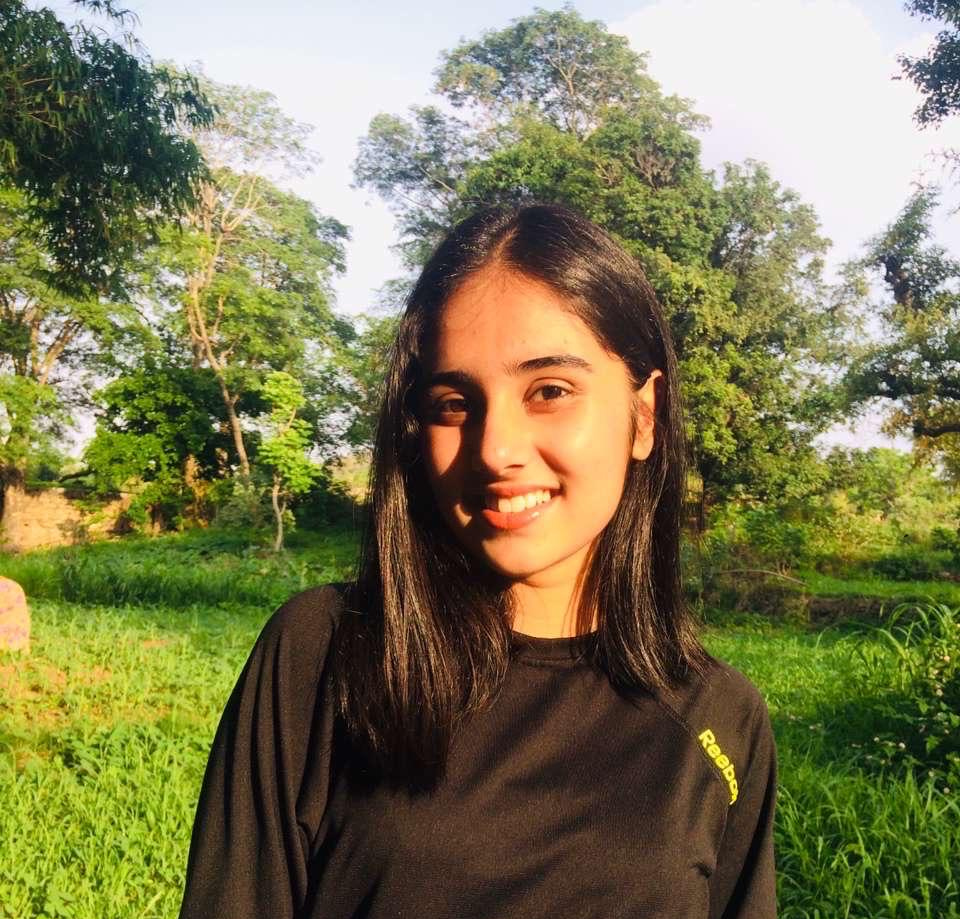
\includegraphics[width=0.35\textwidth]{Assets/SuryanshiRanawat.png}
\end{figure}

\noindent \textbf{Name:} Suryanshi Ranawat \\
\textbf{Location:} Udaipur \\
\textbf{Languages:} English, Hindi \\
\textbf{Contact:} 6377722486 \\
\textbf{Email:} \href{mailto:suryanshi.23bce11634@vitbhopal.ac.in}{suryanshi.23bce11634@vitbhopal.ac.in}

\vspace{0.3cm}

\noindent I am currently pursuing a B.Tech in Computer Science and Engineering. I have a strong interest in Artificial Intelligence, Machine Learning, and data-driven problem solving. I have worked on projects such as an AI Disease Detection Platform and a Crop Disease Detection System, which focus on applying AI and machine learning techniques to solve real-world problems in healthcare and agriculture.

My areas of interest include Artificial Intelligence, deep learning, predictive modeling, and intelligent automation systems. I am particularly interested in exploring how AI can be used to build innovative solutions that improve healthcare, agriculture, and decision-making systems.

%--- Ujjwal Mishra ---
\newpage
\subsection*{Ujjwal Mishra}

\begin{figure}[H]
    \centering
    
\includegraphics[width=0.35\textwidth]{Assets/UjjwalMishra.png}
\end{figure}

\noindent \textbf{Name:} Ujjwal Mishra \\
\textbf{Location:} Delhi \\
\textbf{Languages:} English, Hindi \\
\textbf{Contact:} 8920153120 \\
\textbf{Email:} \href{mailto:ujjwal.23bec10079@vitbhopal.ac.in}{ujjwal.23bec10079@vitbhopal.ac.in}

\vspace{0.3cm}

\noindent I am currently pursuing a B.Tech in Electronics and Communication Engineering (ECE). I have a strong interest in electronics systems, embedded technologies, and communication networks. I have worked on projects such as a Mobile Network Jammer and a Hexa-Octal Firefighting Drone, which focus on applying engineering concepts to develop practical solutions for safety and communication-related challenges.

My areas of interest include embedded systems, wireless communication, robotics, and intelligent electronic systems.

In addition to my technical interests, I possess keen leadership abilities and strong teamwork skills, which help me effectively collaborate and manage project responsibilities. My goal is to continue developing advanced technological solutions that contribute to innovation, safety, and efficient communication systems.

%--- Medhansh Singh Kushwaha ---
\newpage
\subsection*{Medhansh Singh Kushwaha}

\begin{figure}[H]
    \centering
    
\includegraphics[width=0.35\textwidth]{Assets/MedhanshSinghKushwaha.png}
\end{figure}

\noindent \textbf{Name:} Medhansh Singh Kushwaha \\
\textbf{Location:} Agra \\
\textbf{Languages:} English, Hindi \\
\textbf{Contact:} 7055333362 \\
\textbf{Email:} \href{mailto:medhansh.23bce11385@vitbhopal.ac.in}{medhansh.23bce11385@vitbhopal.ac.in}

\vspace{0.3cm}

\noindent I am currently pursuing a B.Tech in Computer Science Engineering (CSE) with a strong interest in web development, full stack technologies, and digital design. I have experience working with HTML, CSS, React.js, Node.js, and MySQL to build responsive and user-friendly web applications.

I am also interested in graphic design and UI/UX, using tools such as Adobe Photoshop, Figma, and Blender to create visual content and interface designs. Currently, I am contributing to a Breast Cancer Detection project, where I apply my development and design skills to support the software and interface aspects of the system.

Along with my technical skills, I possess strong creativity, problem-solving ability, and teamwork skills, and I aim to develop innovative technology solutions that contribute to meaningful real-world applications.

%--- Soumyadeep Chakravarti ---
\newpage
\subsection*{Soumyadeep Chakravarti}

\begin{figure}[H]
    \centering
    
\includegraphics[width=0.35\textwidth]{Assets/SoumyadeepChakravarti.png}
\end{figure}

\noindent \textbf{Name:} Soumyadeep Chakravarti \\
\textbf{Location:} Delhi \\
\textbf{Languages:} English, Hindi \\
\textbf{Contact:} 9599059229 \\
\textbf{Email:} \href{mailto:soumyadeep.23bai11250@vitbhopal.ac.in}{soumyadeep.23bai11250@vitbhopal.ac.in}

\vspace{0.3cm}

\noindent I am currently pursuing a B.Tech in Computer Science and Engineering with a specialization in Artificial Intelligence. I have a strong interest in Artificial Intelligence, Machine Learning, and systems programming. I have worked on projects such as Jarvis, a C-based AI personal assistant that integrates local language models for intelligent interaction, and PyProbe, a tool for exploring Python's internal memory structures and object layouts.

My areas of interest include Artificial Intelligence, deep learning, and systems-level software development. I am particularly interested in exploring how AI can be combined with efficient low-level programming to build intelligent assistants, advanced tooling, and scalable AI systems.

\end{document}
